%\documentclass[a4paper,prd,twocolumn,nofootinbib,superscriptaddress,floatfix]{revtex4}
\documentclass[prd,twocolumn,nofootinbib,showpacs]{revtex4-1}

%\usepackage{amsmath,amssymb}
\usepackage{cancel}
\usepackage{graphicx}
\usepackage{epsfig}
\usepackage{amsmath,amsfonts,amssymb}
\usepackage{natbib}
\usepackage[utf8]{inputenc}
\usepackage[T1]{fontenc}
\usepackage[english]{babel}
\usepackage{hyphenat}
\hyphenation{mate-mática recu-perar}
\bibliographystyle{unsrtnat}
\usepackage{tabularx} % extra features for tabular environment
\usepackage{amsmath}  % improve math presentation
\usepackage{blindtext}
\usepackage{enumitem}
\usepackage{xcolor}
\usepackage{graphicx} % takes care of graphic including machinery
\usepackage{graphics} 
\usepackage{float}
%\usepackage[margin=1in,letterpaper]{geometry}% decreases margins
%\usepackage{cite} % takes care of citations

\usepackage{lipsum}
\usepackage{mwe}
%\usepackage[affil-it]{authblk}
\graphicspath{{images/}}
\usepackage{cases}
\usepackage[final]{hyperref} % adds hyper links inside the generated pdf file
\usepackage{epstopdf}
\DeclareMathOperator{\sign}{sign}
\begin{document}

%\linenumbers

\title{Equilibrium of a Spherical Pendulum by Energy Control}

\author{N. Teixeira  nº 75494}

\affiliation{Departamento de F\'{\i}sica, Instituto Superior T\'ecnico, Universidade de Lisboa, Lisboa, Portugal}
%\begin{document}

\begin{abstract}
In this paper a successful equilibrium method for the spherical pendulum at the vertical position is studied. We have applied two types of controls to the pivot of the pendulum. One of the  controls increases or decreases the polar angle variation by moving the pivot in the polar direction, the other type of control alters the azimuthal angle of the pendulum by exercing a radial movement on the pivot based on the difference of energy between the unstable vertical position ($\theta=0$, $\theta'=0$) and the actual time. The numerical method applied, fourth order Runge-Kutta, didn't have a negative influence in the final result since no anomalies were found.
\end{abstract}

\maketitle

\section{Introduction}
\subsection{1D Control method}\label{1D}



\noindent Stabilization of a pendulum around it's vertical position in one dimension by energy control was studied by Astrom \& Furuta \cite{Furtura} and R. Dilão \cite{Dilao}. 

\begin{figure}[H]
    \centering
    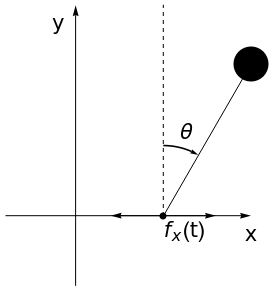
\includegraphics[width=0.25\textwidth]{pend1d.png}
    \caption{Equilibrium of the pendulum in one dimension. The function $f_x(t)$ controls the horizontal movement of the pivot.  $\theta$ is bigger than $0$ when clockwise.}
    \label{fig:1D}
\end{figure}


Considering the setup in Fig. (\ref{fig:1D}), $\theta$ is the polar angle, the angle measured from the vertical where the positive sign is clockwise, $l$ is the length of the pendulum. Since the pivot of the pendulum is mobile, we can seperate the decription of the problem in two parts, the position of the pivot, $f_x(t)$, and the position of the mass of the pendulum relative to it's pivot, 

\begin{equation}
x(t)=f_x(t)+ l \sin{\theta}(t),
\label{x1d}
\end{equation}
\begin{equation}
y(t)= l \cos{\theta}(t).
\label{y1d}
\end{equation}



\noindent In cartesian coordinates the Lagrangian is written as:
\begin{equation}
    \mathcal{L}=\frac{1}{2}m\left(\dot{x}^2+\dot{y}^2\right)-m g y,
    \label{l1d}
\end{equation}
\noindent substituting in with Eqs. (\ref{x1d}) and (\ref{y1d}). We have the following equation  of motion for $\theta$,

\begin{equation}
    \ddot{\theta}-\frac{g}{l}\sin{\theta}=-u(t)\cos{\theta},
    \label{theta1d}
\end{equation}
where $u(t)=\ddot{f_x}/l$.

\par We are interested in controlling the position of the pendulum in the pivot frame. One of the methods to balance the pendulum is by controlling the energy. The expression for the derivative of the energy can thus be obtained,
\begin{equation}
    \mathcal{H}=\frac{\dot{\theta}^2}{2}+ \frac{g}{l}\cos{\theta}
    \label{energia1d}
\end{equation}
\begin{equation}
 \frac{d\mathcal{H}}{dt}=\dot{\theta}\left(\ddot{\theta}-\frac{g}{l}\sin{\theta}\right)   
\end{equation}
Substituting Eq. (\ref{theta1d}),in the derivative we get.

\begin{equation}
    \frac{d\mathcal{H}}{dt}=-u(t) \,\dot{\theta}\,\cos{\theta}
    \label{control1d}
\end{equation}
Equation (\ref{control1d}) exhibits  the strategy of the control  method used. Fixing $u(t)$, in case the coefficient $\dot{\theta}\cos{\theta}$ is bigger than 0, the energy gets lowered, otherwise is raised. We can thus invert the effect of the product $\dot{\theta}\cos{\theta}$ and only base our control function $u(t)$, so that it depends only on the  difference of the energies between the pendulum, in the vertical position with its energy given by $E_1=+g/l$, and the energy at the actual time given in Eq. (\ref{energia1d}). This way the control function $u(t)$ can be expressed as,
\begin{equation}
    u(t)=-\mu  \sign\left({E_1-E}\right) \sign{(\dot{\theta} \cos{\theta})},
    \label{u1d}
\end{equation}
where, $\mu>0$ is an external control parameter.
\par When the energy $E$ is lower (higher) than $E_1$, the control function $u(t)$ raises (lowers) the current energy $E$ until $E=E_1$ so that the pendulum remains in an equilibrium position in it's unstable vertical position. 

\subsection{2D Control Method}
A 2D control method was implemented for the spherical pendulum regarding the information of Sec. (\ref{1D}). In this case, similarly with Eq. (\ref{x1d}) the position of the pendulum with a 2D control function is given by,
\begin{equation}
x(t) =f_x(t)+ l \sin{\theta}\cos{\phi}   
\end{equation}
\begin{equation}
  y(t)=f_y(t)+l\sin{\theta}\sin{\phi} ,
\end{equation}
\begin{equation}
    z(t)=l \cos{\theta},
\end{equation}
 $\theta$ is the azimuthal angle and $\phi$ is the polar angle. The equations of motion become,
\begin{equation}
\scalebox{0.80}[1]{$\ddot{\theta}-\frac{g}{l}\sin{\theta}- \dot{\phi}^2\, \cos{\theta}\,\sin\theta =-\cos{\theta} (\cos{\phi}\, u_x(t)+ \sin{\phi}\, u_y(t)),$}
\label{teta2d}
\end{equation}
\begin{equation}
  \scalebox{0.78}[1]{$\ddot{\phi}\sin^2{\theta} +2 \, \dot{\phi} \,\dot{\theta}\sin{\theta} \cos{\theta}= -\sin{\theta}\sin{\phi}\, u_x(t) + \sin{\theta}\cos{\phi} \,u_y(t),$}
  \label{phi2d}
\end{equation}
with $u_x(t)=\ddot{f_x(t)}/l$ and $u_y(t)=\ddot{f_y(t)}/l$, the control functions for respectively the $x$ and $y$ direction. The variation of energy can be determined as it has been done in Sec. (\ref{1D}),
\begin{equation}
    \mathcal{H}=\frac{\dot{\theta}^2}{2}+\frac{1}{2}\dot{\phi}^2 \sin^2{\theta}+\frac{g}{l}\cos{\theta}
\end{equation}

Substituing Eqs. (\ref{teta2d}) and (\ref{phi2d}) in the derivative of the energy in order to time, we obtain,

\begin{align}
    \frac{d\mathcal{H}}{dt}=&-\dot{\phi}\,\sin{\theta}(-\sin{\phi}\,u_x(t)+\cos{\phi}\,u_y(t)) \nonumber \\ 
    &-\dot{\theta}\,\cos{\theta}(\cos{\phi}\,u_x(t)+\sin{\phi}\,u_y(t))
    \label{dhdt2d}
\end{align}
Equation (\ref{dhdt2d}) displays the geometric relationship between, $u_x(t)$ and $u_y(t)$.
\par In case,
\begin{equation}
   \Vec{o}(t)= \begin{cases}
    u_x(t)=o(t) \cos{\phi}, &\\
    u_y(t)=o(t) \sin{\phi}, &
    \end{cases}
\end{equation}
this is, if $u_x(t)$ and $u_y(t)$ are aligned with the  projection of the radial versor, $\hat{e_r}$, with the $xy$ plane, Eq. (\ref{dhdt2d}) reduces to very similar form of Eq. (\ref{control1d}) with the exception that $\Vec{o}$ is a 2D variable and not 1D. This way, the control function $o(t)$ monitors the energy regarding the azimuthal variation, it's rotation around $\hat{e_{\phi}}$ versor. 
\par In case,
\begin{equation}
    \Vec{s}(t)=\begin{cases}
    u_x(t)=-s(t) \sin{\phi}, &\\
    u_y(t)=s(t) \cos{\phi}, &
    \end{cases}
\end{equation}
so that $u_x(t)$ and $u_y(t)$ are aligned with the polar versor, $\hat{e_{\phi}}$, the term, in Eq. (\ref{dhdt2d}) proportional to $\dot{\theta}$ goes to 0 leaving the the control function $s(t)$ to modify the energy regarding the polar angle variation $\phi'$, in other words its rotation about Z axis. We can then implement the two types of control by summing vectorially each acceleration component, 

\begin{equation}
\Vec{u}(t)=\begin{cases}
    u_x(t)=o(t) \cos{\phi} -s(t) \sin{\phi}, &\\
    u_y(t)=o(t) \sin{\phi}+ s(t) \cos{\phi}. &
    \end{cases}
    \label{accel}
\end{equation}
\par In order to control the pendulum so that it remains balanced with it's pivot, ($\theta=0$,  $\dot{\theta}=0$), the strategy was use the control function  $s(t)$ to deaccelerate the rotation of the pendulum, until $\dot{\phi}=0$. This way, $s(t)$ has the following form, 
\begin{equation}
s(t)=\nu \sign{(\dot{\phi}\sin{\theta})}, 
\label{controlv2d}
\end{equation}
with $\nu >0$ as an external parameter to the problem.
\noindent At the same time that the control mechanism in Eq. (\ref{u1d}) is applied to raise or lower the energy $E$ to the final state ,$E_1=+g/l$, by modifying the radial position of the pivot. The control function $o(t)$ has then the following form,
\begin{equation}
 o(t)=-\mu  \sign\left({E_1-E}\right)\sign{(\dot{\theta} \cos{\theta})}, 
 \label{controlu2d}
\end{equation}

\noindent with, $\mu>0$ as a external control parameter. 
\par Fig (\ref{fig:control2d}) ilustrates an examples of the 2D control functions $\Vec{o}(t)$ and $\Vec{s}(t)$. 
\begin{figure}[H]
    \centering
    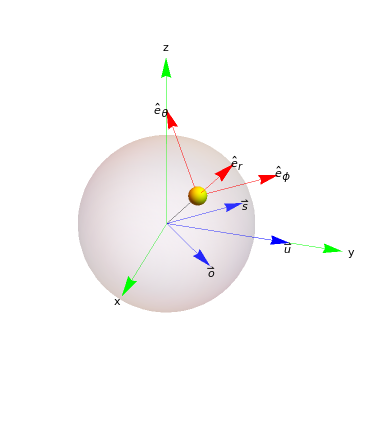
\includegraphics[width=0.3\textwidth]{Excontrolo4_1.png}
    \caption{Example of control functions $\Vec{o}(t)$ and $\Vec{s}(t)$ displayed as  blue arrows, to balance the yellow pendulum around it's unstable vertical position. The axis $x$, $y$, $z$ are displayed in green and the spherical versors, $\hat{e_{\phi}}$, $\hat{e_{\theta}}$, $\hat{e_r}$ in red. The control  $o(t)$  has the function of raising the $z$ position of the pendulum to it's unstable vertical position, $z=l$, and the control $s(t)$ is responsible for slowing the rotation around $Z$ axis, $\dot{\phi}$.} 
    \label{fig:control2d}
\end{figure}
\section{Numerical Method}
The numerical method applied in order to solve the system was a fourth order Runge-Kutta method \cite{Rungekutta}, for both $\dot{\phi}$ and $\dot{\theta}$. Having a timestep, $\Delta t$ and a max number of iterations $Nmax$, this method is applied when we have a generic function $x$ such that,
\begin{equation}
\dot{x}=g(x,t),
\end{equation}
the next iteration of $x$ by the fourth order Runge-Kutta method is given by,
\begin{equation}
x_{n+1}=x_n+\frac{\Delta t}{6}(k1+2 \,k2+2\,k3+k4).
\end{equation}
The $k$ coefficients are given by,
\begin{equation}
k_1=   g(t,x_n ),
\end{equation}


\begin{equation}
    k_2= g\left(t+\frac{\Delta t}{2},x_n+\frac{k_1}{2}\right),
\end{equation}

\begin{equation}
        k_3= g\left(t+\frac{\Delta t}{2},x_n+\frac{k_2}{2}\right),
\end{equation}

\begin{equation}
      k_4= g(t+\Delta t,x_n+k_3).
\end{equation}
Associating Eq. (\ref{teta2d}) with $\ddot{\theta}=g_{\dot{\theta}}$ and Eq. (\ref{phi2d}) with $\ddot{\phi}=g_{\dot{\phi}}$ we can obtain the next iteration of  $\dot{\theta}$ and $\dot{\phi}$.  The functions to integrate by the Runge-Kutta method can be written in the following way,
\begin{align}
g_{\dot{\theta}}=&\cos{\theta_n}\,(\sin\theta_n \,\dot{\phi_n}^2- \cos{\phi_n}\, u_{x_n}- \sin{\phi_n}\, u_{y_n}) +\nonumber \\
&\frac{g}{l}\sin{\theta_n},
\end{align}
\begin{equation}
g_{\dot{\phi}} =\frac{2 \, \dot{\phi_n} \,\dot{\theta_n} \cos{\theta_n} -\sin{\phi_n}\, u_{x_n}+ \cos{\phi_n} \,u_{y_n}}{\sin{\theta_n}}, 
\end{equation}
\begin{equation}
g_{\theta}=\dot{\theta_n},
\end{equation}
\begin{equation}
    g_{\phi}=\dot{\phi_n}.
\end{equation}

\noindent We can apply the Runge-Kutta method to Eqs. (\ref{accel}) as done with $\theta$ and $\phi$. This way, the position of the mobile pivot, the functions $f_x$, $f_y$,  can be known along side it's derivatives, $\dot{f_x}$ and $\dot{f_y}$. In the end, with the proper set of initial values, and applying the method until the last iteration, $Nmax$, a solution to the problem may be determined so that the pendulum remains in a balanced position.

\section{Results}
Figs.$\,$(\ref{fig:teta})-(\ref{fig:labref}) display the result from a simulation with S.I. units and the following parameters: $l=1$ m, $m=1$ Kg, $g=1$ m/s\textsuperscript{2}, $\mu$,$\nu=0.3$ s\textsuperscript{-2},$\phi_0'=2$ s\textsuperscript{-1}, $\theta_0=\frac{3\pi}{4}$ , $\Delta t=0.001$ s, $Nmax=20000$,
and 
\begin{equation}
    \phi_0,f_{x_0},f_{y_0},\dot{f_{x_0}},\dot{f_{y_0}}=0. 
\end{equation}
\begin{figure}[H]
    \centering
    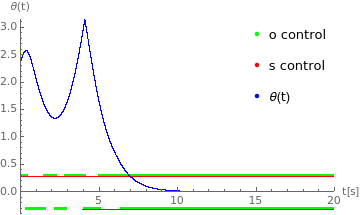
\includegraphics[width=0.40\textwidth]{Estabilizacaoteta1.png}
    \caption{In this figure the variation of $\theta$ with time is displayed in blue. After the simulation starts, the pendulum takes approximetely 10 seconds to balance around the pivot. The $o(t)$ and $s(t)$ control functions are displayed respectively in green and red. It can be seen that $s(t)$ initially is assymetric becouse the pendulum is rotating around the Z axis, but with time, this rotation decreases, and it's average equals 0 to correct any deviation from equilibrium, $\phi'=0$.}
    \label{fig:teta}
\end{figure}

\begin{figure}[H]
    \centering
    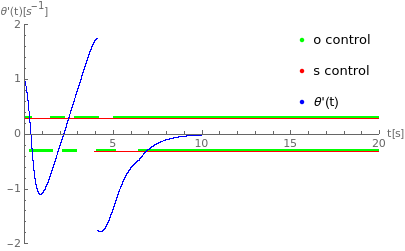
\includegraphics[width=0.40\textwidth]{Estabilizacaotetalinha1.png}
    \caption{This figure displays the variation of $\theta'$ with time in blue. This function has a great oscilation, but it decreases to $0$ after $t=10$ s where the pendulum remains in equilibrium until the end of the simulation.}
    \label{fig:tetalinha}
\end{figure}

\begin{figure}[H]
    \centering
    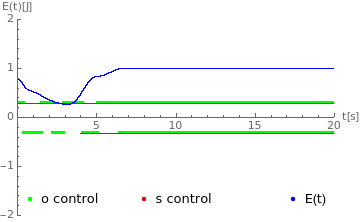
\includegraphics[width=0.40\textwidth]{Estabilizacaoenergy1.png}
    \caption{This figure displays the variation of energy marked with blue points. The control $o(t)$ initially oscillates with a certain frequency, so that the pendulum has enough energy to reach the top. After the pendulum reaches equilibrium , $o(t)$ oscilates very rapidly toward 0, similarly to the $s(t)$ control in the balance stage, in order to correct any deviation from stability.}
    \label{fig:energy}
\end{figure}

\begin{figure}[H]
    \centering
    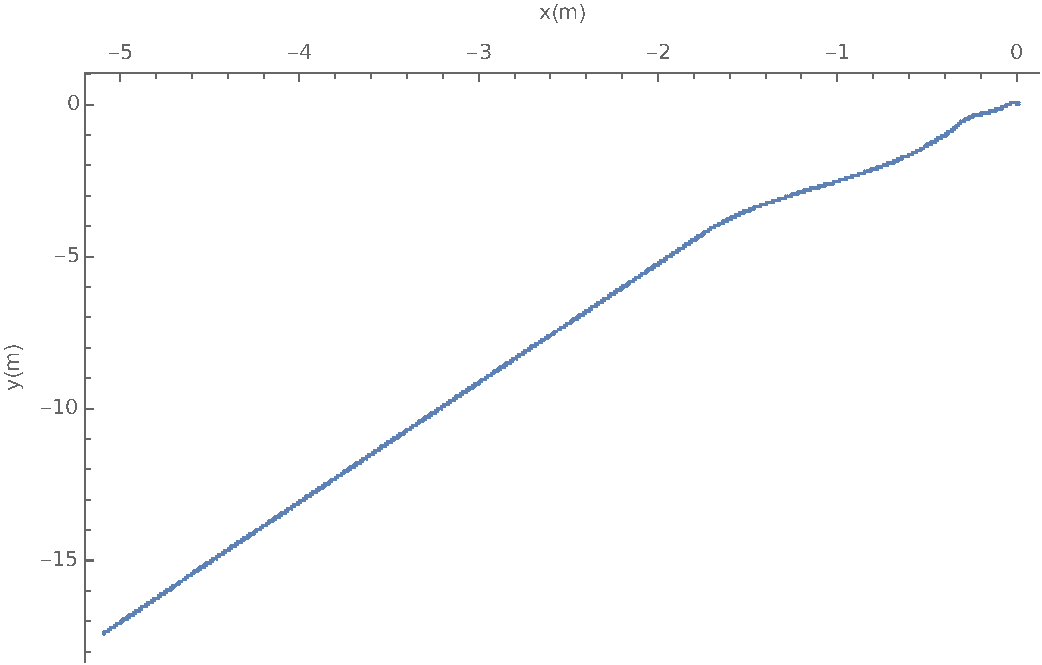
\includegraphics[width=0.45\textwidth]{Estabilizacaopos1.pdf}
    \caption{In this figure the trajectory of the pivot, $f_x(t)$ and $f_y(t)$ is displayed in blue. Most of the rotational movement in the beginning of the simulation is transfered to the pivot so that the center of the pendulum remains in a constant drift after it reaches the equilibrium, this is, approximately, the moment when the slope $dy/dx$ is constant.}
    \label{fig:pos}
\end{figure}

\begin{figure}[h]
    \centering
    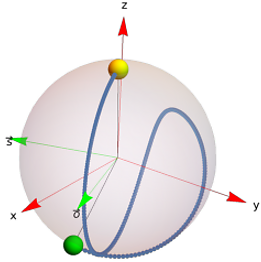
\includegraphics[width=0.35\textwidth]{Estabilizacao1.png}
    \caption{This figure displays the trajectory from the pivot frame. The green pendulum is the initial state and the yellow pendulum is the final state of the simulation. As it can be seen, initially the rotation around the Z axis is reduced and afterwards the pendulum reaches the balanced state where $z=l$. The vectors $\Vec{s}(t)$ and $\Vec{o}(t)$ correspond to the forces per length that the pivot is subjected.}
    \label{fig:pivotref}
\end{figure}

\begin{figure}[H]
    \centering
    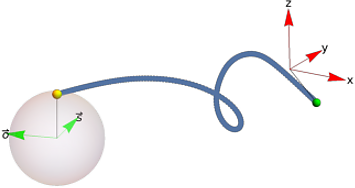
\includegraphics[width=0.4\textwidth]{Estabilizacaotraj1.png}
    \caption{This figure displays the trajectory from the laboratory frame. As in Fig. (\ref{fig:pivotref}), the initial state corresponds to the initial state and the yellow pendulum corresponds to the moment the pendulum becomes balanced. It is possible to see that when the pendulum arrives its balanced stance, it remains with the same velocity to not break it's stability.}
    \label{fig:labref}
\end{figure}
\section{Conclusions}

In this work a spherical pendulum control was studied so that after a certain time a vertical balance was reached by  controlling the movement of it's pivot. It was seen in the previous sections that the requirement to obtain such an equilibrium was to make two types of control, one to stop the rotation around the Z axis and another to modify the energy of the pendulum to reach the state where the pendulum is balanced, $\theta=0$ and $\theta'=0$.
\par Figs.$\,$(\ref{fig:teta})-(\ref{fig:labref}) show that such balance was possible along with the determination of the trajectory of the pivot. The system was successfully represented, with no instabilities, and the numerical method applied, the fourth order Runge-Kutta \cite{Rungekutta}, remained consistent and without significant errors throught the simulation.
Eventhough it was possible to achieve a balance, it was not done under the minimal time nor effiency. A detailed stability analysis of the parameters $\mu$ and $\nu$ can be done to study the effects of each parameter in the dynamics and stability of the system. 
\par In the future, a more realistic model may be studied by introducing air resistance and aerodynamic coefficients to study the different types of cases where this method to achieve balance is possible and in which situations. 
Besides an energy control method, it is possible that other methods may also decrease the time to reach a balance or increase the range of stability and therefore maximize the efficiency to equilibrate a pendulum in it's unstable vertical position.



\begin{thebibliography}{99}

\bibitem{Furtura}
 Åström, Karl Johan, and Katsuhisa Furuta. "Swinging up a pendulum by energy control." Automatica 36.2 (2000): 287-295.
 \bibitem{Rungekutta}
Süli, Endre; Mayers, David, An Introduction to Numerical Analysis, Cambridge University Press,(2003): ISBN 0-521-00794-1 

 \bibitem{Dilao}
 R. Dilão, "Uma Introdução à Teoria dos Sistemas Dinâmicos e do Caos",IST 31.2 (2018): 330-335, .
  %%CITATION = HEP-PH/0607298;%%
  %51 citations counted in INSPIRE as of 26 Sep 2013

\end{thebibliography}

\end{document}
